\documentclass[12pt]{scrartcl} %or scrbook

\usepackage{xcolor}
\definecolor{darkred}{rgb}{0.75,0,0}
\definecolor{darkblue}{rgb}{0,0,0.5}
\definecolor{darkgreen}{rgb}{0,0.5,0}
\definecolor{darkergreen}{rgb}{0,0.75,0}
\definecolor{darkmagenta}{rgb}{0.55,0,0.55}
\definecolor{left}{HTML}{041832}
\definecolor{secondary}{HTML}{241024}

\usepackage[colorlinks=true,
		     urlcolor=darkblue,
		     citecolor=darkergreen,
		     linkcolor=darkblue,
		     plainpages=false,
		     pdfpagelabels]{hyperref}

\setlength{\parindent}{0pt}
\setlength{\parskip}{.25cm}

\usepackage{graphicx}

%If you want to typeset code, use minted (requires
%some additional setup)
%\usepackage{minted}

%If you want to typeset algorithms, use algorithm2e:
%\usepackage[boxed,slide,linesnumbered]{algorithm2e}

\title{Some Project}
\subtitle{Computer Science II Project}
\author{Joe Schmoe\\
        \href{mailto:foo@email.com}{foo@email.com} \\
        Jane Schmoe\\
        \href{mailto:foo@email.com}{foo@email.com} \\
        Department of Computer Science \& Engineering\\
        University of Nebraska---Lincoln\\
}

\date{Fall 2525 \\
      Version 1.x
}

\begin{document}

\maketitle
\thispagestyle{empty}

\vfill

\begin{abstract}
[Provide a short abstract of this document here]
\end{abstract}

\newpage
\clearpage
\setcounter{page}{1}
\section*{Revision History}

\begin{tabular}{|l|l|l|l|}
\hline
Version & Description of Change(s) & Author(s) & Date \\
\hline
1.0 & Initial draft of this design document & Joe Schmoe & 2525/01/01 \\
\hline
1.1 & Typo and grammar fixes & Jane Schmoe & 2525/01/02 \\
\hline
\end{tabular}

\newpage
\tableofcontents

\newpage
\section{Introduction}

[Provide a short introduction to this document, the project and the context in which it is being developed.  This document needs to conform to the 
IEEE 1016 standard \cite{IEEE1016} (this is how you use citations).]

\subsection{Purpose of this Document}

[Describe the purpose of this document; the goal(s) that its content are intended to achieve]

\subsection{Scope of the Project}

[Describe the scope of the project, what features and functionality it covers (at a high-level).  Describe the problem statement and context in which this project is being developed.  Who is it for, what is it for, etc.?  You may also explicitly indicate what is not within the scope--other potential pieces of the overall project that are not covered by this document]

\subsection{Definitions, Acronyms, Abbreviations}

\subsubsection{Definitions}

[Define any terms that require a definition--domain specific terms, non-standard terms, or terms that are used in non-standard ways]

\subsubsection{Abbreviations \& Acronyms}

[Define all abbreviations and acronyms used in this document here.  This relieves you of the need to define such things within the context of the document itself and provides an easy reference for the reader.]

\begin{description}
  \item[ACM] Association for Computing Machinery
  \item[IEEE] Institute of Electrical and Electronics Engineers
  \item[UAV] Unmanned Aerial Vehicle
\end{description}
  
\section{Overall Design Description}
  
[Provide an overall summary/description of the project.  Identify the major design components, technologies, etc.]
  
\subsection{Alternative Design Options}

[If applicable, describe and discuss alternative design options that you considered and discuss why they were not chosen.  What advantages and disadvantages do the alternatives provide and what advantage/disadvantages do the chosen design elements provide.  Provide some justification for why the chosen elements? advantages/disadvantages outweighed the alternatives]

\section{Detailed Component Description}

[Provide an introduction to this section here]

\subsection{Database Design}

[This section will be used to detail your database schema design (Phase III).  In earlier phases this section may be omitted or a short note indicating that details will be provided in a subsequent revision of this document.]

\subsubsection{Component Testing Strategy}

[This section will describe your approach to testing this particular component.]

\subsection{Class/Entity Model}

[This section should detail your Java classes--their state, interface and how they relate to each other.  It is highly recommended that you document these elements using tables, UML diagrams, and other visually-informative methods.  Figures and tables should have proper captions and be referenced in the main text just like in Figure \ref{figure:uav}.  You should provide subsections to organize your presentation as applicable.]

\begin{figure}
\centering
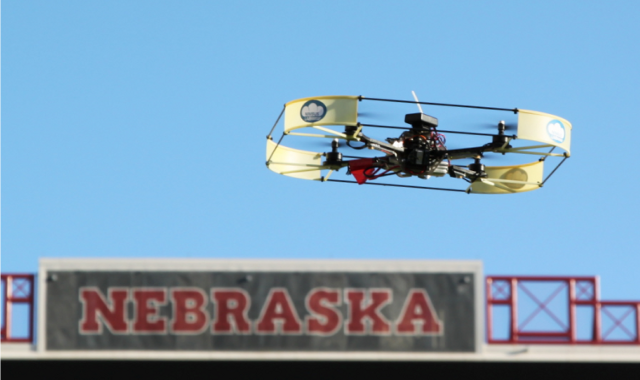
\includegraphics[scale=1.0]{uavsUNL}
\caption{A UAV (Unmanned Aerial Vehicle) soars above Memorial Stadium.  Figures should be numbered and properly captioned.}
\label{figure:uav}
\end{figure}

\subsubsection{Component Testing Strategy}

[This section will describe your approach to testing this particular component.  Describe any test cases, unit tests, or other testing components or artifacts that you developed for this component.  What were the outcomes of the tests?  Did the outcomes affect development or force a redesign?]

\subsection{Database Interface}

[This section will be used to detail phase IV where you modify your application to read from a database rather than from flat files.  This section will detail the API that you designed--how it conformed to the requirements, how it worked, other tools or methods that you designed to assist, how it handles corner cases and the expectations or restrictions that you?ve placed on the user of the API.  In earlier phases this section may be omitted or a short note indicating that details will be provided in a subsequent revision of this document.  An example table is presented
as Table \ref{table:assignmentPerformance}.]

\begin{table}
\centering
\caption{Average Performance on Assignments; on-time vs. late and individual vs partners.  In general, captions for Tables should appear above the table.}
\label{table:assignmentPerformance}
\begin{tabular}{|l|p{1.5cm}|p{1.5cm}|p{1.5cm}|p{1.5cm}|p{1.5cm}|p{1.5cm}|p{1.5cm}|}
\hline
~ & 1 & 2 & 3 & 4 & 5 & 6 & 7 \\
\hline
On-time	& 93.16\% (78.46\%)	& 88.06\% (72.31\%)	& 87.89\% (67.69\%)	& 89.37\% (56.92\%) & 83.42\% (29.23\%) & 88.40\% (53.85\%) & 74.56\% (75.38\%) \\
\hline
Late & 88.75\% (12.31\%) & 85.28\% (20.00\%) & 70.32\% (15.38\%) & 90.40\% (15.38\%) & 82.74\% (44.62\%) & 94.22\% (15.38\%) & N/A \\
\hline
Diff & \color{red}{4.42\%} & \color{red}{2.79\%} & \color{red}{17.57\%} & \color{green}{1.03\%} & \color{red}{0.68\%} & \color{green}{5.82\%} & - \\
\hline
Individual & NA	& 88.43\% (73.85\%) & 82.32\% (33.85\%) & 87.22\% (27.69\%) & 86.40\% (23.08\%) & 82.67\% (26.15\%) & ~\\
\hline
Pairs & NA & 83.55\% (18.46\%) & 86.22\% (49.23\%) & 91.00\% (46.15\%) & 78.53\% (49.23\%) & 92.83\% (46.15\%) & ~\\
\hline
Diff & NA & \color{red}{4.88\%} & \color{green}{3.90\%} & \color{green}{3.78\%} & \color{red}{7.87\%} & \color{green}{10.16\%}	& ~\\
\hline
\end{tabular}
\end{table}

\subsubsection{Component Testing Strategy}

[This section will describe your approach to testing this particular component.  Describe any test cases, unit tests, or other testing components or artifacts that you developed for this component.  What were the outcomes of the tests?  Did the outcomes affect development or force a redesign?]

\subsection{Design \& Integration of Data Structures}

[This section will be used to detail phase V where you design an original data structure and integrate it into your application.  In earlier phases this section may be omitted or a short note indicating that details will be provided in a subsequent revision of this document?]

\subsubsection{Component Testing Strategy}

[This section will describe your approach to testing this particular component.  Describe any test cases, unit tests, or other testing components or artifacts that you developed for this component.  What were the outcomes of the tests?  Did the outcomes affect development or force a redesign?]

\subsection{Changes \& Refactoring}

[During the development lifecycle, designs and implementations may need to change to respond to new   requirements, fix bugs or other issues, or to improve earlier poor or ill-fitted designs.  Over the course of this project such changes and refactoring of implementations (to make them more efficient, more convenient, etc.) should be documented in this section.  If not applicable, this section may be omitted or kept as a placeholder with a short note indicating that no major changes or refactoring have been made.]

\section{Additional Material}

[This is an optional section in which you may place other materials that do not necessarily fit within the organization of the other sections.]

\addcontentsline{toc}{section}{Bibliography}
\nocite{*}
\bibliographystyle{plain}
%\bibliographystyle{elsarticle-harv}
\bibliography{bibliography}

\end{document}